\providecommand{\mainpath}{..} % Command to retrieve the path of the main file. It must be defined before documentclass.

\documentclass[\mainpath/main]{subfiles}
\begin{document}

\chapter{Integration Strategy} % First chapter
\label{IntegrationStrategy}

% Command to be executed after the starting of every chapter
\setmyfancystyle
% ----------------

In this chapter the integration strategy will be described. In the \autoref{IntegrationStrategy:EntryCriteria} the prerequisites for the tests will be presented. The \autoref{IntegrationStrategy:ElementsToBeIntegrated} is dedicated to the required components to be integrated in the system to execute some tests.\\
Finally in the sections \ref{IntegrationStrategy:IntegrationTestingStrategy} and \ref{IntegrationStrategy:SequenceofComponent_FunctionIntegration} the strategy used to test the integrations will be discussed, paying attention to the order.

\section{Entry Criteria}
\label{IntegrationStrategy:EntryCriteria}
The criteria which are required to perform each test are easy. The involved components (and eventually needed program stubs) must be developed and fully tested before executing the integration test.\\
In addition, for some test, further preconditions may be required. These prerequisites will not be described here, but in the \autoref{IndividualStepsAndTestDescription}, dedicated to test's description.

\section{Elements to be Integrated}
\label{IntegrationStrategy:ElementsToBeIntegrated}
First of all, no further components need to be integrated to perform integration tests.\\
Then, to perform the tests described in the following pages, all the components of the system need to be implemented. Furthermore, it is not required that all the components must be implemented before executing the first integration test: in the \autoref{IntegrationStrategy:SequenceofComponent_FunctionIntegration:SoftwareIntegrationSequence} the order of implementation is well-presented focusing both on the subsystems and on the reasons for the required order.

\section{Integration Testing Strategy}
\label{IntegrationStrategy:IntegrationTestingStrategy}
We have decided to test our system's interactions with a bottom-up approach. In the \autoref{IntegrationStrategy:SequenceofComponent_FunctionIntegration} it is possible to see the components' order of implementation defined by us with specific criteria. As soon as two components are available, the tests associated to their interactions have to be applied. Before starting the development of the following part of the system, all the tests should be successful.\\ Obviously, to perform some tests, we need to use a \textit{non-available} component (it has not been implemented yet): to simulate this components we will use some particular program stubs, if any, and they will be described in detail in the \autoref{ProgramStubsAndTestDataRequired}.

\section{Sequence of Component/Function Integration}
\label{IntegrationStrategy:SequenceofComponent_FunctionIntegration}
In this section we point out the features related to the order of the components' development. Which is our order of implementation? Why do we need to develop the component \textit{A} before \textit{B}? These two questions are fully discussed from now.

\subsection{Software Integration Sequence}
\label{IntegrationStrategy:SequenceofComponent_FunctionIntegration:SoftwareIntegrationSequence}
The \textquotedblleft subsystems\textquotedblright\ of \textit{myTaxiService} are two, both important.\\
The \textit{Client and User Handler} has the specific role to bind the users' requests to the corresponding services on the system by enqueueing the request on the dispatcher. Then it is able to show the results or to perform the following interactions of the involved service.\\
To handle these operations it has three components, with the names \textit{Authentication}, \textit{ServiceShow} and \textit{ClientInterface}\footnote{To have a brief description of each of them read the Design Document.}. In the \autoref{IntegrationStrategy:SequenceofComponent_FunctionIntegration:SoftwareIntegrationSequence:ClientHandlerSequence} the order of implementation is shown\footnote{According to the Design Document the reader may expect to see all the interfaces of the Client and User Handler. To simplify the representation all the interfaces and the classes have been grouped and inserted into the related component.}.

\begin{figure}[h]
	\centering
	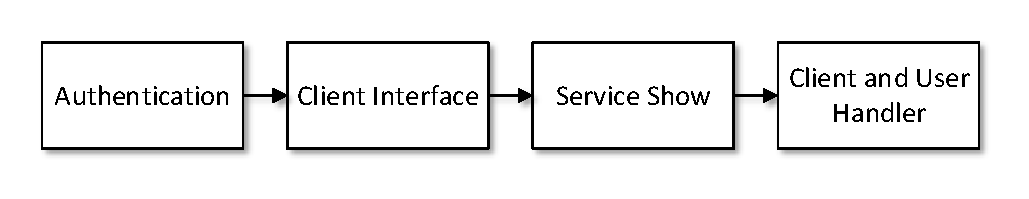
\includegraphics[width=\textwidth]{ClientHandlerSequence}
	\caption{Integration Sequence of Client and User Handler}
	\label{IntegrationStrategy:SequenceofComponent_FunctionIntegration:SoftwareIntegrationSequence:ClientHandlerSequence}
\end{figure}

The \textit{Ride Allocator} handles everything that is related to a ride, so the taxy drivers' queues, their assignments and the identification of their positions (by GPS coordinates or an address).\\
A more precise description is available in the Design Document, as usual, whereas here we are interested only in the implementation order shown in \autoref{IntegrationStrategy:SequenceofComponent_FunctionIntegration:SoftwareIntegrationSequence:RideAllocatorSequence}

\begin{figure}[h]
	\centering
	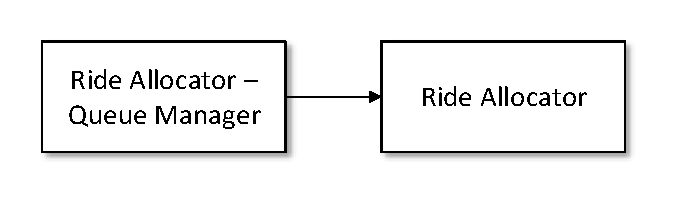
\includegraphics[width=\textwidth]{RideAllocatorSequence}
	\caption{Integration Sequence of Ride Allocator}
	\label{IntegrationStrategy:SequenceofComponent_FunctionIntegration:SoftwareIntegrationSequence:RideAllocatorSequence}
\end{figure}

The interactions and the integration inside these two subsystems are not tested in this project phase, but when the single components are implemented. In fact, each component is tested as soon as its first implementation has been completed and until all the tests are successful the development can not be considered done.\\
This kind of tests are defined in a dedicated document, called \textit{Unit Test Plan Document}, not available now for \textit{myTaxiService}.

\subsection{Subsystem Integration Sequence}
\label{IntegrationStrategy:SequenceofComponent_FunctionIntegration:SubsystemIntegrationSequence}
In this section we will present the global interactions between the \textit{myTaxiService}'s core subsystems and we will define all the integration tests and their order.\\
In the \autoref{IntegrationStrategy:SequenceofComponent_FunctionIntegration:SoftwareIntegrationSequence:IntegrationTestOrder} we can see the components' implementation order, as we suppose it is better: first of all the DBMS, then, in this order, all related to data checking or handling, to the users, to the security, to the rides and, finally, the dispatcher (the most important component in our system).

\begin{figure}[h]
	\centering
	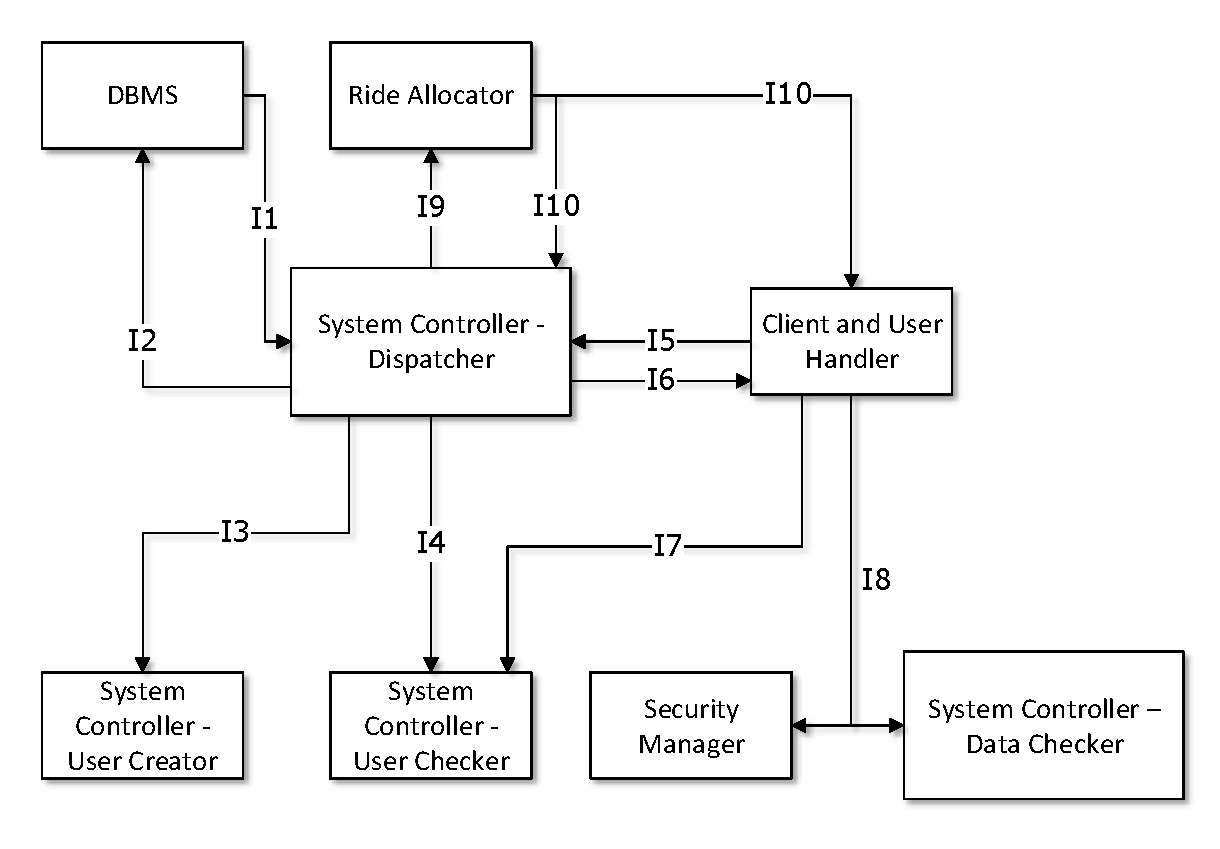
\includegraphics[width=\textwidth]{IntegrationTestOrder}
	\caption{Integration Test Order}
	\label{IntegrationStrategy:SequenceofComponent_FunctionIntegration:SoftwareIntegrationSequence:IntegrationTestOrder}
\end{figure}

\clearpage

\textbf{Integration tests.}\\
\begin{table}[h]
	\centering
	\begin{tabular}[!ht]{c|p{12cm}c}
		ID & Integration test & \\ \hline
		% Created DBMS
		I1 &  \centering DBMS $\rightarrow$ System Controller - Dispatcher  & \\ \hline
		I2 & \centering System Controller - Dispatcher $\rightarrow$ DBMS  & \\ \hline
		% Created User Creator
		I3 & \centering System Controller - Dispatcher $\rightarrow$ User Creator   & \\ \hline
		% Created User Checker
		I4 & \centering System Controller - Dispatcher $\rightarrow$ User Checker   & \\ \hline
		% Created Client and User Handler
		I5 & \centering Client and User Handler $\rightarrow$ System Controller - Dispatcher   & \\ \hline
		I6 & \centering Client and User Handler $\rightarrow$ User Checker , Security Manager   & \\ \hline
		% Created Data Checker and Security Manager
		I7 & \centering Client and User Handler $\rightarrow$ System Controller - Data Checker , Security Manager   & \\ \hline
		% Created Ride Allocator
		I8 & \centering System Controller - Dispatcher $\rightarrow$ Ride Allocator   & \\ \hline
		I9 & \centering Ride Allocator $\rightarrow$ System Controller - Dispatcher , Client and User Handler   & \\ \hline
	\end{tabular}
\end{table}

\end{document}